\documentclass{article}
\usepackage{tikz}
\usepackage[margin = 0.5in]{geometry}
\usepackage{verbatim}

\begin{comment}
10
18
\end{comment}

\begin{document}

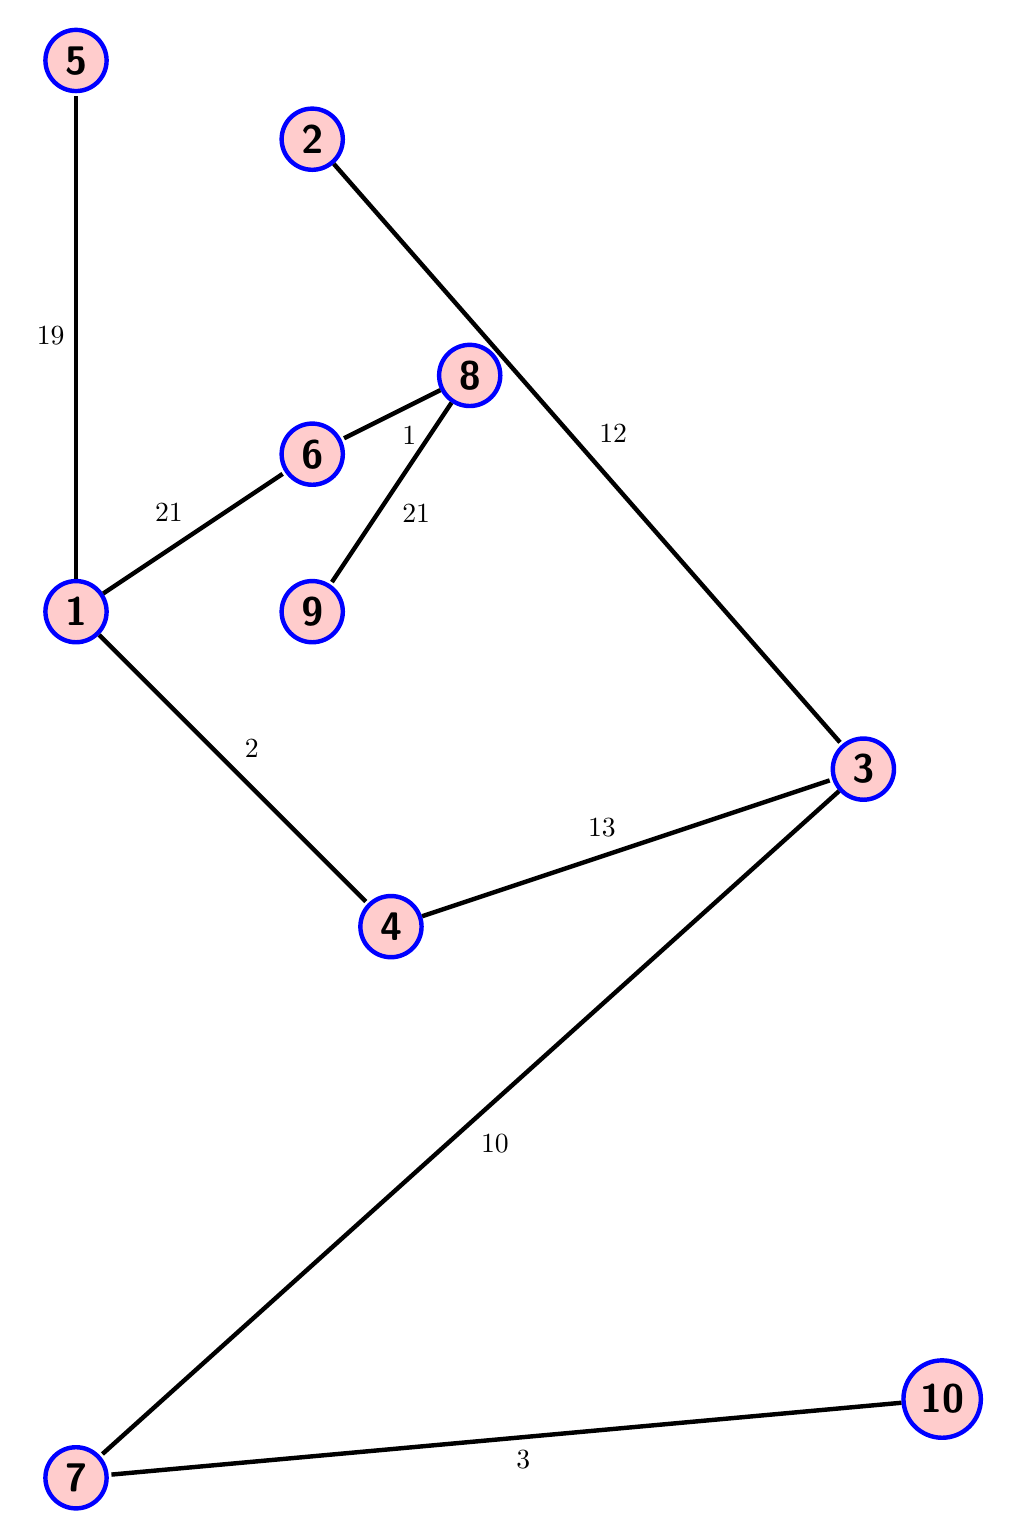
\begin{tikzpicture}[shorten >=1pt, auto, node distance=3cm, ultra thick]

   \begin{scope}[every node/.style={circle,draw=blue,fill=red!20!,font=\sffamily\Large\bfseries}]
    \node (v1) at (-2,2) {1};
    \node (v2) at (1,8) {2};
    \node (v3) at (8,0) {3};
    \node (v4) at (2,-2) {4};
    \node (v5) at (-2,9) {5};
    \node (v6) at (1,4) {6};
    \node (v7) at (-2,-9) {7};
    \node (v8) at (3,5) {8};
    \node (v9) at (1,2) {9};
    \node (v10) at (9,-8) {10};
   \end{scope}
   \begin{scope}[every edge/.style={draw=black,ultra thick}]
   \end{scope}
\draw (v1) edge node{2} (v4);
\draw (v4) edge node{13} (v3);
\draw (v3) edge node{10} (v7);
\draw (v10) edge node{3} (v7);
\draw (v2) edge node{12} (v3);
\draw (v1) edge node{19} (v5);
\draw (v1) edge node{21} (v6);
\draw (v8) edge node{1} (v6);
\draw (v8) edge node{21} (v9);
\end{tikzpicture}

\end{document}
